\subsection{Линейный график технологического процесса}

Для планирования сроков выполнения работ и анализа их взаимосвязей применяется метод сетевого планирования. Он позволяет представить процесс разработки программного средства в виде ориентированного графа, отражающего последовательность выполнения задач и зависимости между ними.

В сетевой модели каждая работа задаётся кодом, включающим номера начального и конечного событий. События фиксируют завершение этапов, а работы описывают переходы между ними. Такой подход позволяет определить критический путь проекта, оценить его длительность и выявить временные резервы.

На основе ранее определённых работ и их трудоёмкости сформированы коды и рассчитаны параметры сетевого графа. Соответствие событий и работ приведено в таблице \ref{tab:work_codes}.

{
\fontsize{10}{10}\selectfont
\setlength{\tabcolsep}{3pt}

\begin{longtable}{|c|p{3cm}|p{3cm}|p{1.5cm}|p{1.5cm}|p{1.2cm}|p{1.2cm}|p{2.9cm}|}
\caption{Соответствие событий и работ}\label{tab:work_codes} \\
\hline
№ & Событие & Работа & Т (ч) & Т (дн) & Код  & Тип & Исполнитель \\ \hline
\endfirsthead

\caption*{Продолжение таблицы \ref{tab:work_codes}}\\ \hline
№ & Событие & Работа & Т (ч) & Т (дн) & Код  & Тип & Исполнитель \\ \hline
\endhead

\hline
\endfoot

\hline
\endlastfoot

1 & Начало работ & Анализ предметной области и существующих решений & 28 & 3.5 & 1-2 & ОН & Аналитик \\ \hline

2 & Завершение анализа предметной области & Формирование требований к системе & 18 & 2.3 & 2-3 & ОН & Аналитик \\ \hline

\multirow{2}{*}{3} & \multirow{2}{*}{\parbox{3cm}{Утверждение технического задания}}
& Проектирование общей архитектуры системы & 40 & 5 & 3-4 & ОН & Инженер \\ \cline{3-8}
& & Подготовка и предобработка данных & 56.0  & 7.0 & 3-6 & ОН & Аналитик \\ \hline

4 & Проектирование общей архитектуры системы завершено & Проектирование структуры данных & 19.6  & 2.5 & 4-5 & ОН & Инженер \\ \hline

5 & Проектирование структуры данных завершено & Реализация модуля сбора и обработки логов & 112 & 14.0 & 5-9 & ОН & Инженер \\ \hline

6 & Подготовка и предобработка данных завершена & Разработка моделей НС для обнаружения аномалий & 67.2 & 8.4 & 6-7 & ОН & Аналитик \\ \hline

7 & Разработка моделей НС завершена & Обучение моделей НС & 50.4 & 6.3 & 7-8 & ОН & Аналитик \\ \hline

8 & Обучение моделей НС завершено & Оценка и сравнение моделей & 28  & 3.5 & 8-10 & ОН & Аналитик \\ \hline

9 & Реализация модуля сбора и обработки логов завершена & Реализация модуля анализа и обнаружения аномалий & 64.0  & 8.0 & 9-10 & ОН & Инженер \\ \hline

10 & Реализация модуля анализа и обнаружения аномалий завершена & Интеграция модели НС в систему & 44.0  & 5.5  & 10-11 & ОН & Инженер \\ \hline

11 & Интеграция модели НС в систему завершена & Настройка взаимодействия компонентов системы & 44.0  & 5.5  & 11-12 & ОН & Инженер \\ \hline

12 & Настройка взаимодействия компонентов системы завершена & Функциональное тестирование & 176  & 22  & 12-13 & ОН & Инженер \\ \hline

13 & Функциональное тестирование завершено & Исправление ошибок и оптимизация & 112.0 & 14.0  & 13-14 & ОН & Инженер \\ \hline

14 & Исправление ошибок и оптимизация завершены & Подготовка документации & 168  & 21 & 14-15 & ОН & Инженер \\ \hline

15 & Завершение проекта & - & -  & - & - & - & - \\ \hline

\end{longtable}
}

Построение модели выполнено в системе ProjectLibre. Исходные данные заданы в соответствии с таблицей \ref{tab:work_codes}. Диаграмма Ганта представлена на рисунке \ref{fig:gantt_chart} и отражает распределение работ во времени.

\begin{figure}
    \centering
    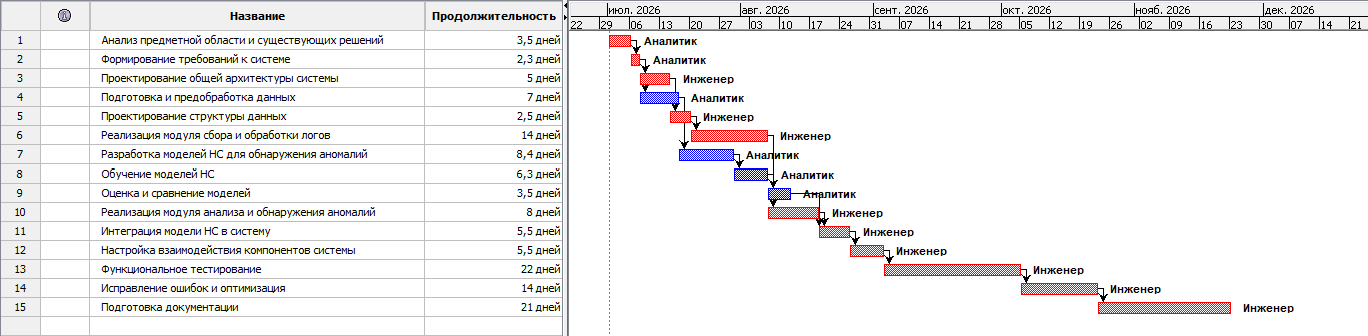
\includegraphics[scale=0.6]{inc/images/gantt_chart}
    \caption{Диаграмме Ганта.}
    \label{fig:gantt_chart}
\end{figure}

Моделирование позволяет определить не только календарные параметры выполнения работ, но и потребность в трудовых ресурсах. Сводные трудозатраты по исполнителям приведены в таблице \ref{tab:labor_costs}.

\begin{table}[h!]
  \centering
  \caption{Трудозатраты по исполнителям}
  \begin{tabular}{|l|r|}
  \hline
  \textbf{Исполнитель} & \textbf{Трудозатраты, часы} \\
  \hline
  Инженер & 780 \\ \hline
  Аналитик & 248 \\ \hline
  \end{tabular}
  \label{tab:labor_costs}
\end{table}

\subsection{Оптимизация ресурсов}

После создания диаграммы Ганта необходимо проанализировать загруженность персонала, чтобы определить возможность перераспределения имеющихся ресурсов и улучшения структуры графика. Свободные ресурсы сотрудников могут быть использованы для помощи в текущих задачах или выполнения других подзадач. 

Загрузка инженера представлена на рисунке \ref{fig:workload_engineer}, аналитика — на рисунке \ref{fig:workload_analyst}.

\begin{figure}[h!]
    \centering
    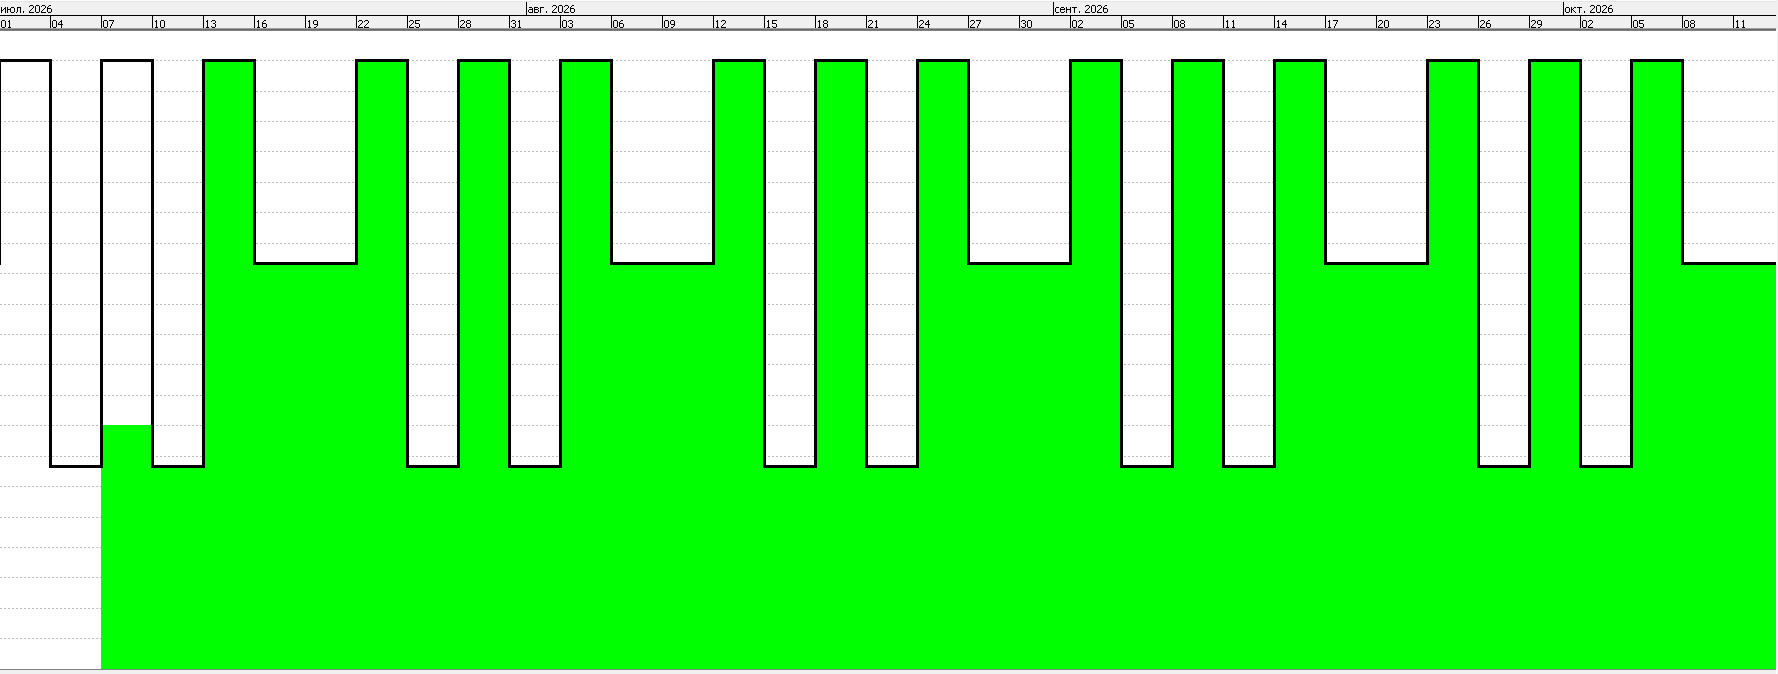
\includegraphics[width=0.5\textwidth]{inc/images/workload_engineer}
    \caption{Загрузка инженера по дням}
    \label{fig:workload_engineer}
\end{figure}

\begin{figure}[h!]
    \centering
    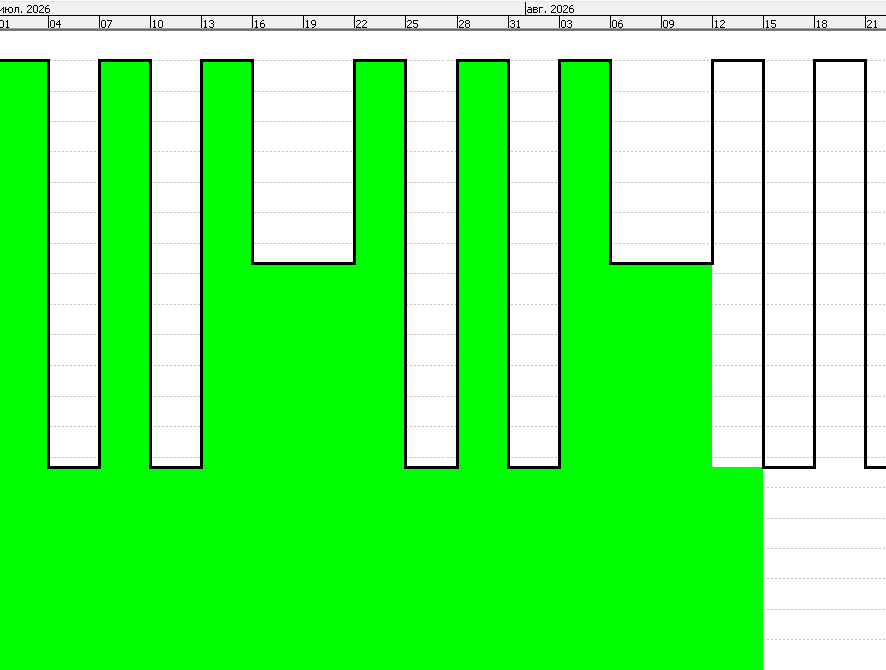
\includegraphics[width=0.5\textwidth]{inc/images/workload_analyst}
    \caption{Загрузка аналитика по дням}
    \label{fig:workload_analyst}
\end{figure}

Анализ показывает, что после 12 августа аналитик не задействован, поскольку его задачи завершены. У инженера наблюдается простой с 1 по 6 июля, обусловленный необходимостью завершения этапа формирования требований. Эти интервалы не подлежат оптимизации в рамках текущей логики процесса. Таким образом, ресурс инженера и аналитика заполнен максимально эффективно в рамках технологического процесса.

\subsection{Сетевой график работ}

Для оценки предпринимаемых мер по отношению к возможным чрезвычайным ситуациям и их затратам необходимо создать сетевую диаграмму и выявить критический путь. Критический путь представляет собой самый длительный маршрут в сетевой диаграмме, включающий работы, не имеющие запаса по времени.

Невыполнение хотя бы одной из задач на критическом пути вовремя приведет к увеличению времени выполнения всего проекта. Это, в свою очередь, повлечёт за собой рост расходов на его осуществление, включая оплату труда, аренду ресурсов и прочие сопутствующие затраты.  

Сетевой график работ проекта представлен на рисунке~\ref{fig:network_diagram}.

\begin{figure}[h!]
    \centering
    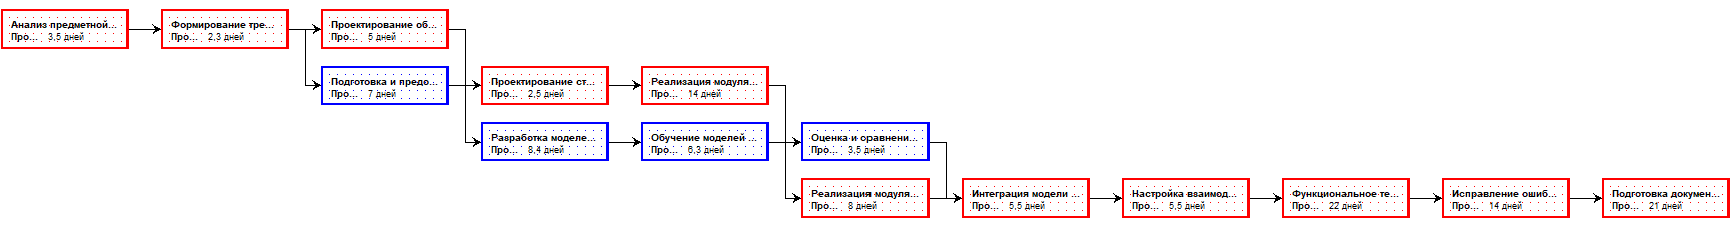
\includegraphics[width=0.85\textwidth]{inc/images/network_diagram}
    \caption{Cетевой график работ}
    \label{fig:network_diagram}
\end{figure}

Длительность критического пути составляет 102 дня, и он проходит через следующие работы:

\begin{enumerate}
    \item анализ предметной области и существующих решений;
    \item формирование требований к системе;
    \item проектирование общей архитектуры системы;
    \item проектирование структуры данных;
    \item реализация модуля сбора и обработки логов;
    \item реализация модуля анализа и обнаружения аномалий;
    \item интеграция модели НС в систему;
    \item настройка взаимодействия компонентов системы;
    \item функциональное тестирование;
    \item исправление ошибок и оптимизация;
    \item подготовка документации.
\end{enumerate}

